\documentclass[conf]{new-aiaa}
%\documentclass[journal]{new-aiaa} %for journal papers
%\documentclass[a4paper]{article}
%\documentclass{homework}

%% Sets page size and margins
%\usepackage[a4paper,top=3cm,bottom=2cm,left=3cm,right=3cm,marginparwidth=1.75cm]{geometry}

%\usepackage[utf8]{inputenc}
\usepackage{graphicx}
\usepackage{amsmath}
\usepackage[version=4]{mhchem}
\usepackage{siunitx}
\usepackage{longtable,tabularx}
\setlength\LTleft{0pt} 
%======================================

% additions
\graphicspath{ {figures/} }
\usepackage{floatrow}
\usepackage{ar}
\usepackage{amstext} % for \text macro
\usepackage{array}   % for \newcolumntype macro
\usepackage{gensymb} % for degree symbol
\newcolumntype{L}{>{$}l<{$}} % math-mode version of "l" column type
\usepackage[numbered,framed]{matlab-prettifier}

\pagestyle{empty}

\definecolor{listinggray}{gray}{0.9}
\definecolor{lbcolor}{rgb}{0.9,0.9,0.9}
\lstset{
backgroundcolor=\color{lbcolor},
    tabsize=4,    
%   rulecolor=,
    language=fortran,
        basicstyle=\mlttfamily,
        upquote=true,
        aboveskip={1.5\baselineskip},
        columns=fixed,
        showstringspaces=false,
        extendedchars=false,
        breaklines=true,
        prebreak = \raisebox{0ex}[0ex][0ex]{\ensuremath{\hookleftarrow}},
        frame=single,
        numbers=left,
        showtabs=false,
        showspaces=false,
        showstringspaces=false,
        identifierstyle=\mlttfamily,
				keywordstyle=\color{blue}\mlttfamily,
				stringstyle=\color{red}\mlttfamily,
				commentstyle=\color[RGB]{34,139,34}\mlttfamily,
				morecomment=[l][\color{magenta}]{\#}
        %keywordstyle=\color[rgb]{0,0,1},
        %commentstyle=\color[rgb]{0.026,0.112,0.095},
        %stringstyle=\color[rgb]{0.627,0.126,0.941},
        %numberstyle=\color[rgb]{0.205, 0.142, 0.73},
%        \lstdefinestyle{C++}{language=C++,style=numbers}’.
}
%\usepackage{titlesec}
%\titleformat*{\paragraph}{\large\bfseries}
%======================================
\title{CE 791 HPC - Assignment 4: Simple MPI}

\author{Andrew Navratil}

\begin{document}

\maketitle

\section*{Part 1. Pi Example}

The pi example program in Fortran was modified to include a timer with MPI\_Wtime and an outer loop to perform 100 trials of 1 million intervals to get a better sense of the Mflops rating.  The number of flops per interval was estimated as 4: 1 for the x assignment multiplication and subtraction, one for the sum assignment addition, and two inside the function call f(a) with one for the division and one for the multiplication and addition.  Code was executed with mpirun on henry2 for 1,2,4, and 8 processors.  Resulting values for Mflops and Time were output to the console and then copied into Matlab code for plotting.

We can see in the plots below that time decreases as number of processors increases - they are inversely proportional.  The Mflops increases linearly with the number of processors, as expected for this embarrassingly parallel problem.

\begin{figure}[H]
	\centering
	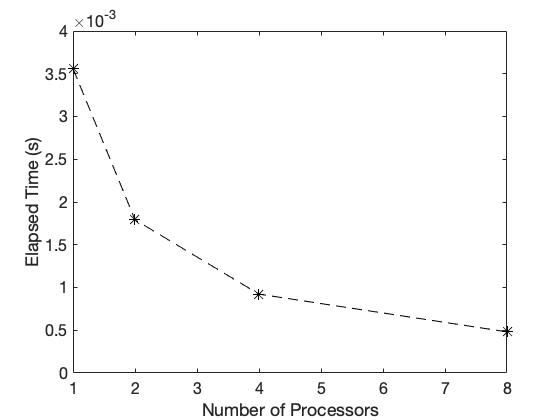
\includegraphics[width=1\columnwidth]{../hw4data/Pi-TimeVsNumProcs.jpg}
	\caption{Execution Time for fpi on henry2}
\end{figure}

\begin{figure}[H]
	\centering
	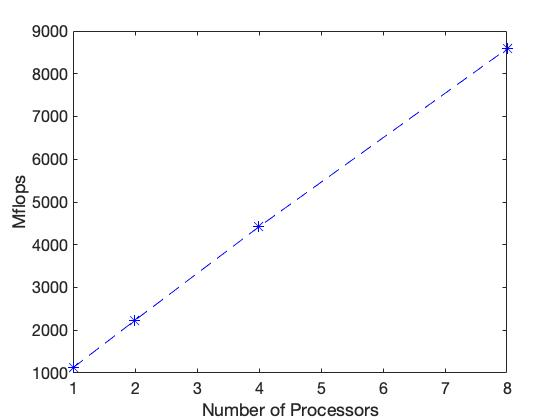
\includegraphics[width=1\columnwidth]{../hw4data/Pi-MflopsVsNumProcs.jpg}
	\caption{Mflops for fpi on henry2}
\end{figure}


\newpage

\section*{Part 2. Water Supply}

The water supply vector program in Fortran was modified to include a timer with MPI\_Wtime, an outer loop to perform 10 trials of 1 million intervals, and MPI\_Reduce with MPI\_MIN.  Resulting values of Mflops were a bit less than the non-parallelized code, more investigation needst to be done into the best way to parallelize all three loops in this code.  Investigation started into MPI\_Gather and could continue there.  Code was executed with mpirun on henry2 for 1,2,4, and 8 processors.  Resulting values for Mflops and Time were output to the console and then copied into Matlab code for plotting.

We can see in the plots below that both time and Mflops degrade as number of processors is increased, showing the need to write a better parallel algorithm for this part of code.

\begin{figure}[H]
	\centering
	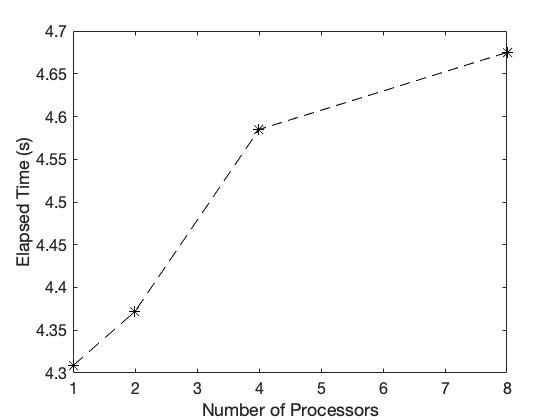
\includegraphics[width=1\columnwidth]{../hw4data/Water-TimeVsNumProcs.jpg}
	\caption{Execution Time for water\_supplyf on henry2}
\end{figure}

\begin{figure}[H]
	\centering
	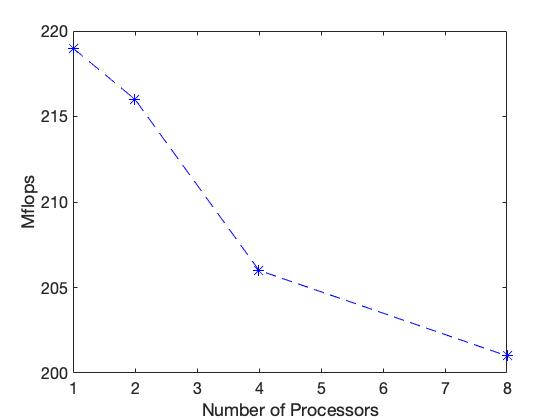
\includegraphics[width=1\columnwidth]{../hw4data/Water-MflopsVsNumProcs.jpg}
	\caption{Mflops for water\_supplyf on henry2}
\end{figure}

%======================================
\newpage
\section*{Fortran Code: Pi}
\lstinputlisting[language=fortran]{../a4/pi_example/fpi.f90}

\newpage

\section*{Fortran Code: Water Supply}
\lstinputlisting[language=fortran]{../a4/water_supply_vector/water_supply.f}

\newpage

\section*{Matlab Code}

\lstset{
  style      = Matlab-editor,
  basicstyle = \mlttfamily,
}
\lstinputlisting{../hw4.m}


\end{document}



